\section{Retrieving Images in Clusters}
\label{sec_introduction}

Many semantic image analysis algorithms, e.g. for image categorization or content detection, require training data on which the relevant features can be learned. Obtaining such training data can be a troublesome task, especially when the training set is created manually and from scratch. If, for example, an algorithm shall be trained to identify and categorize kinds of food, one would have to think of all possible kinds of food, search for corresponding images and divide them into homogeneous groups. \\
A good place to search for images are online photo communities like Flickr\footnote{https://www.flickr.com/}, which provide vast amounts of collaboratively tagged images. These communities are also called folksonomies\index{Folksonomy}, i.e. socially indexed collections.
Although folksonomies can be good sources for training data owing to the semantic metadata that tags provide, several problems exist: First of all, annotations are often of poor quality, since anyone can tag anything with no existing control mechanisms. Secondly, one can only search for a specific term, and will obtain images for all of the term's meanings. However, this way the retrieval is limited to only those images which are annotated with the exact term as a tag. The various semantic relations to other terms are not exploited. Furthermore, the images are usually of a very large visual diversity, which is often not desired. \\

This work presents a tool whose main aim is to create homogeneous groups of semantically and visually similar pictures for a given topic, in order to aid with the laborious assembly of training and test data sets. The main challenges encountered are the homonymy\index{Homonymy} of keywords (the fact that one word can have multiple meanings), the low quality of tags and other annotations, as well as the consideration of both semantic and visual information about a picture.

\subsection{Clustered Tree Nodes Approach}
The tool has been implemented as a Python web application, using WordNet\footnote{http://wordnet.princeton.edu/}\index{WordNet} for semantic image analysis, SimpleCV\footnote{http://www.simplecv.org/} for visual image analysis and Flask\footnote{http://flask.pocoo.org/} together with Bootstrap\footnote{http://getbootstrap.com/} for the frontend presentation.

\begin{figure}[h]
\centering
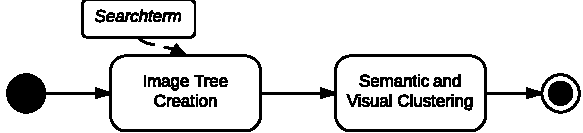
\includegraphics[]{images/search_process_highlevel.pdf}
\caption{The two main phases of the clustered image search}
\label{fig_overallprocess}
\end{figure}

It provides ready-to-use semantically and visually homogeneous image clusters for a given topic, or search term. This is achieved in 2 major phases: First, spanning a tree of subordinate terms of the topic and retrieving related images by their keywords for each node of the tree. Second, clustering the images by their predominant keywords as well as by colors and edge structure. Figure \ref{fig_overallprocess} illustrates these two main phases of the tool.

\subsection{Web Interface}

\begin{figure}[!htb]
  \minipage{0.49\textwidth}
    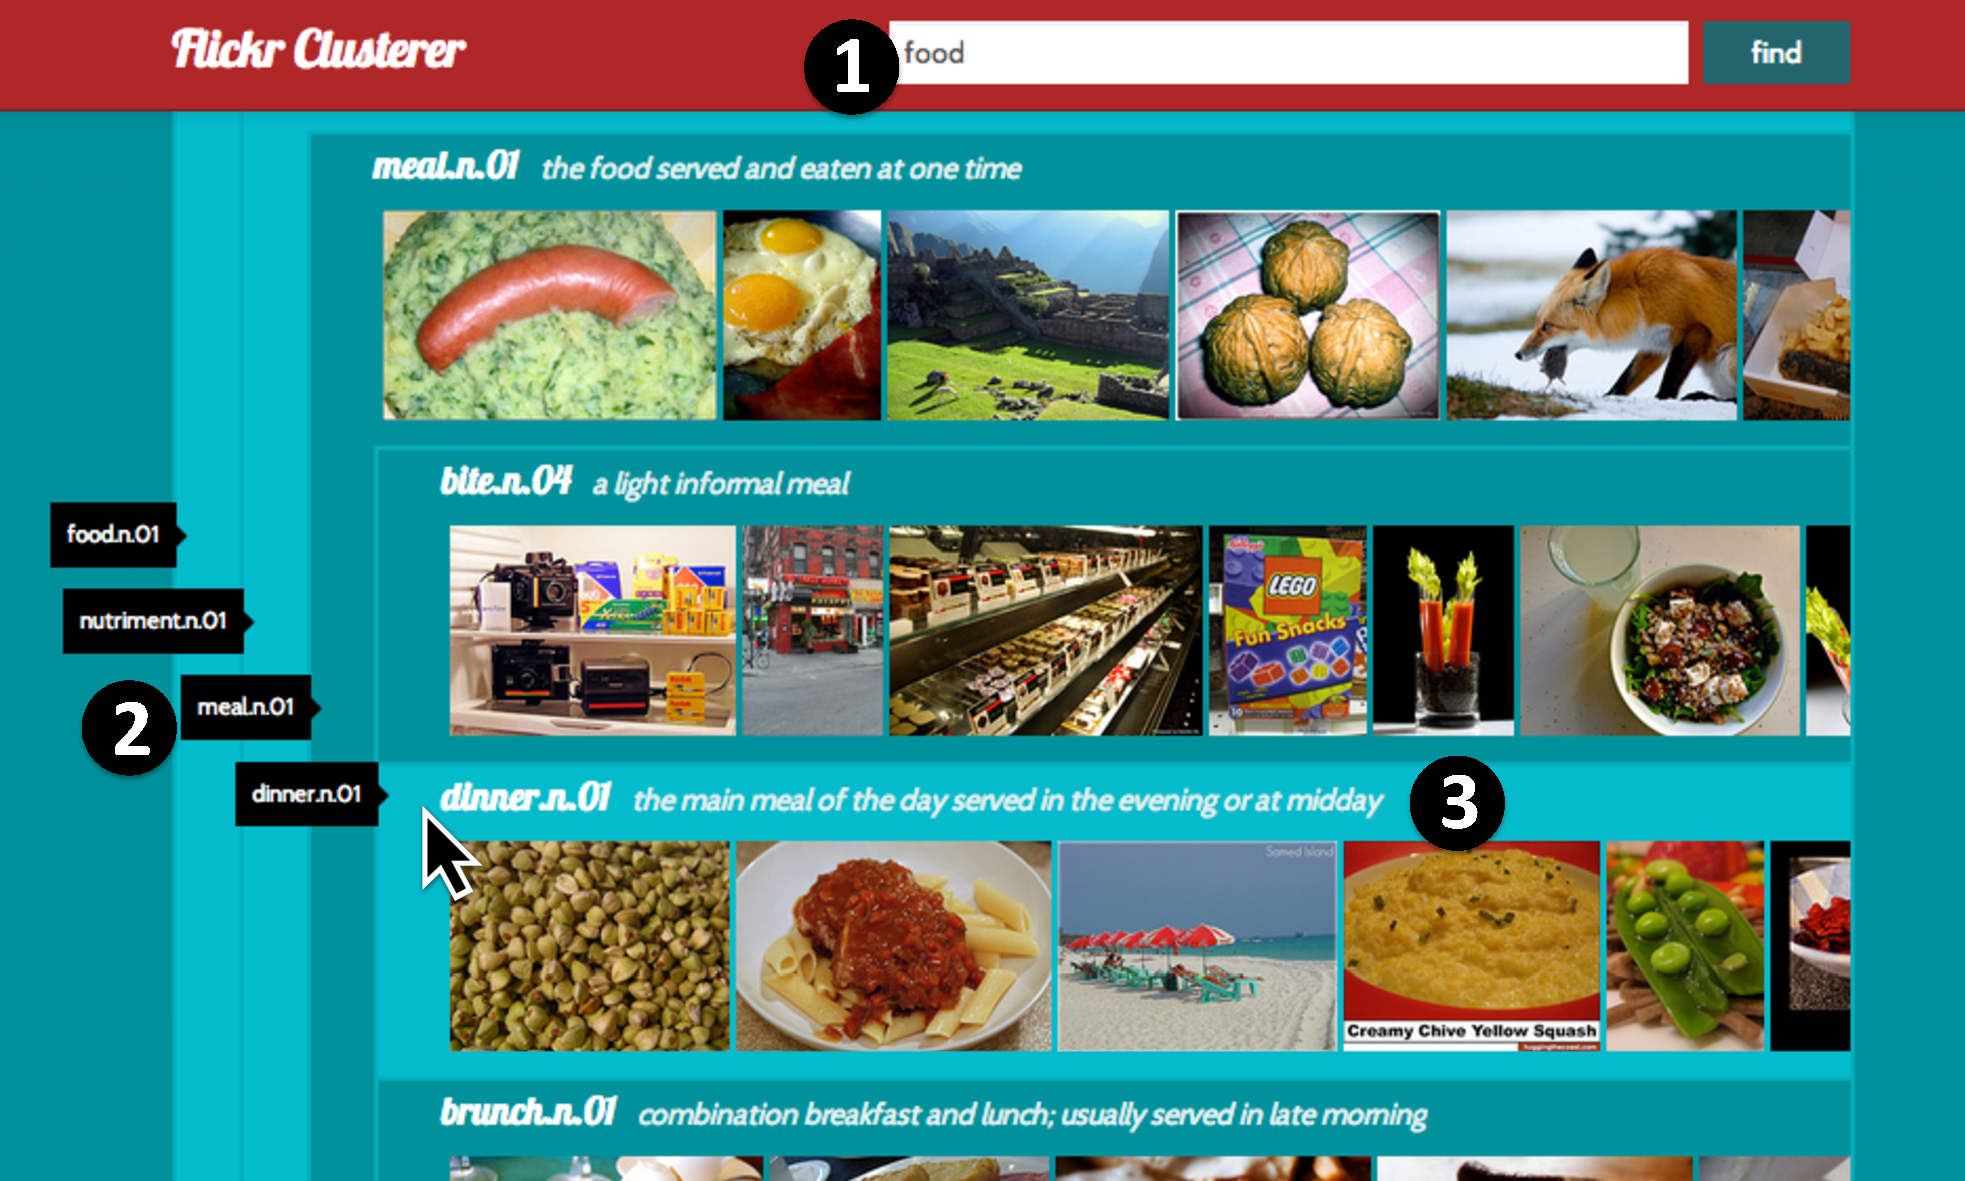
\includegraphics[width=\linewidth]{images/webfrontend-screenshot_1.pdf}
    \caption{Overview of the web interface with search field (1), semantic hierarchy (2) and image preview for each subordinate term (3)}\label{fig_webinerface_1}
  \endminipage\hfill
  \minipage{0.49\textwidth}
    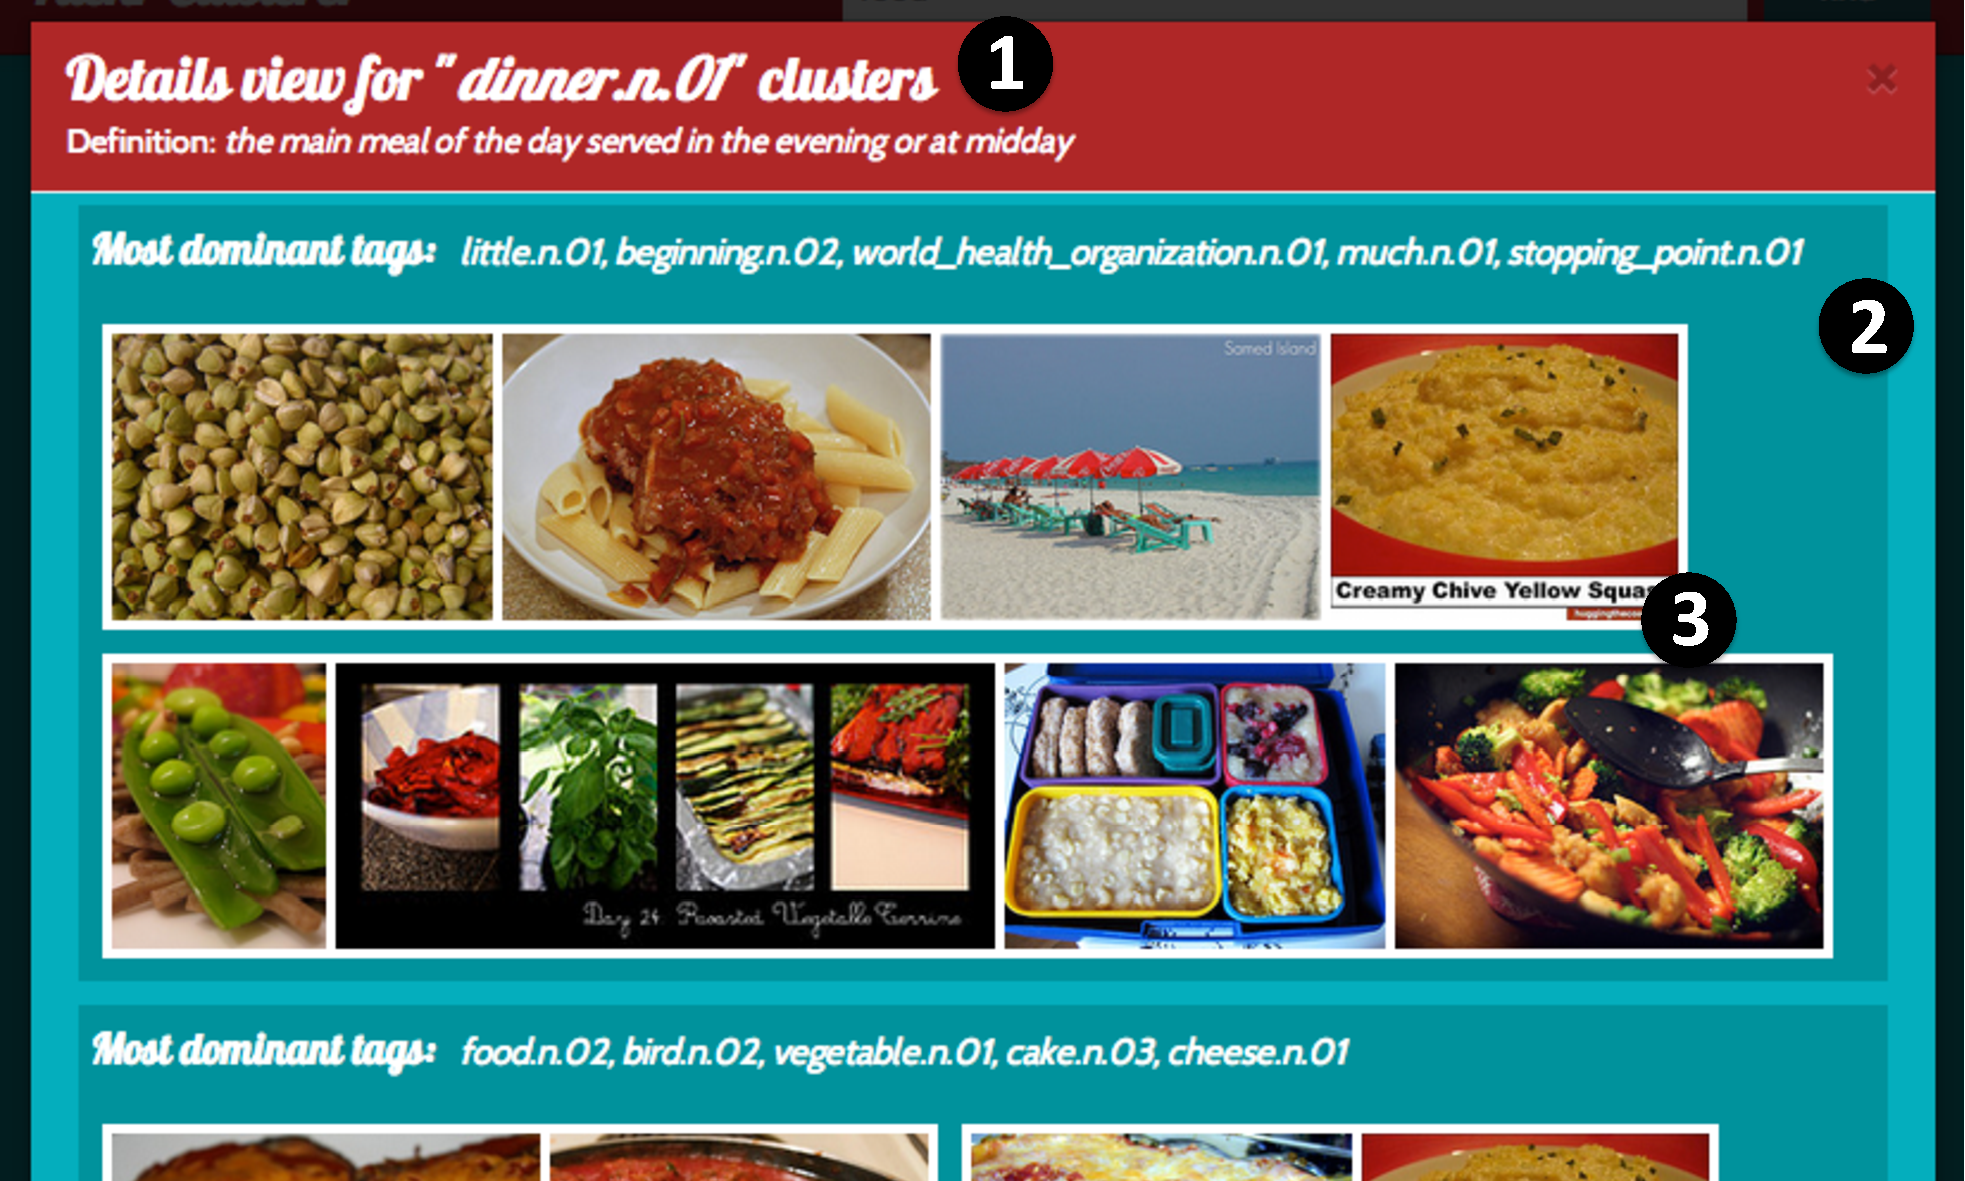
\includegraphics[width=\linewidth]{images/webfrontend-screenshot_2.pdf}
    \caption{Details view for one node with its definition (1), semantic clusters grouped on cyan background (2) and visual clusters grouped on white background (3)}\label{fig_webinerface_2}
  \endminipage\hfill
\end{figure}

After users enter a search term on the web interface (Figure \ref{fig_webinerface_1}, Item 1), they are be presented with a result tree, or, to be exact, with one result tree for each meaning of the term.
All subordinate terms are then recursively found and added to the trees as nodes.
As Item 2 \ref{fig_webinerface_1} shows, this hierarchy is displayed when hovering over the image rows.
Each row shows a preview of the images found for the term represented by this particular node (Item 3). \\
All images for a node can be seen in the \emph{details view} (Figure \ref{fig_webinerface_2}), which is opened by clicking on the images of that node.
This view includes the definition of the subordinate term represented by this node (Item 1)
and shows the images in more finegrained clusters.
The dark cyan background groups semantically similar images (Item 2), i.e. those which have many tags in common. The most common shared tags for each semantic subcluster are also shown.
Within the semantic clusters, the white containers group visually similar images (Item 3). 

\bigskip

After giving an overview of Related Work in chapter 2, we present how we analyze the image annotations and the user's search term to retrieve relevant images in chapter 3. The methods applied to cluster the images semantically and visually are described in chapter 4. Chapter 5 explains how we evaluate our approach, while the evaluation results are discussed in chapter 6. At last, chapter 7 gives ideas for improvement and possible future work.
